\documentclass{article}

% Short communications of approximately 3000 words are also accepted. 
% These papers should contain no more than two figures, two tables, and thirty references. 
% A short abstract of fewer than 200 words is acceptable.

% Bibliography
\usepackage{natbib}
\bibpunct{(}{)}{;}{a}{}{;}

\usepackage[english]{babel}

% Use 'It was found that something is something (Name 1234)' style
\setcitestyle{authoryear,open={},close={}}

% Affiliations
\usepackage{authblk}
\title{The error when inferring phylogenies with incipient species by a Birth-Death model}
% \subtitle{Should protracted speciation be incorporated in phylogenetic tree construction methods?}

\author[1]{Rich\`el J.C. Bilderbeek}
\author[1]{Rampal S. Etienne}
\affil[1]{Groningen Institute for Evolutionary Life Sciences, University of Groningen, Groningen, The Netherlands}

% Load my functions
% The functions used

% My first function, kept for nostalic reasons
\newcommand{\sayhello}{hello and howdy!}

% Making a note
\newcommand\note[1]{\textcolor{green}{\todo{#1}}}

% From https://tex.stackexchange.com/a/98034
\newcommand*\mean[1]{\overline{#1}}

% From https://tex.stackexchange.com/a/101138
% \newcommand\reallywidetilde[1]{\ThisStyle{%
%   \setbox0=\hbox{$\SavedStyle#1$}%
%   \stackengine{-.1\LMpt}{$\SavedStyle#1$}{%
%     \stretchto{\scaleto{\SavedStyle\mkern.2mu\AC}{.5150\wd0}}{.6\ht0}%
%   }{O}{c}{F}{T}{S}%
% }}

% Adapted from 'mean', use 'reallywidetilde'
% \newcommand*\median[1]{\reallywidetilde{#1}}

\newcommand*\median[1]{\widetilde{#1}}

%%%%%%%%%%%%%%%%%%%%%%%%%%%%%%%%%%%%%%%%%%%%%%%%%%%%%%%%%%%%%%%%%%%%%%%%%%%%%%%%
% Create the TikZ picture for fig:experiment
%%%%%%%%%%%%%%%%%%%%%%%%%%%%%%%%%%%%%%%%%%%%%%%%%%%%%%%%%%%%%%%%%%%%%%%%%%%%%%%%
\newcommand{\CreateTikzFigureExperiment} {

  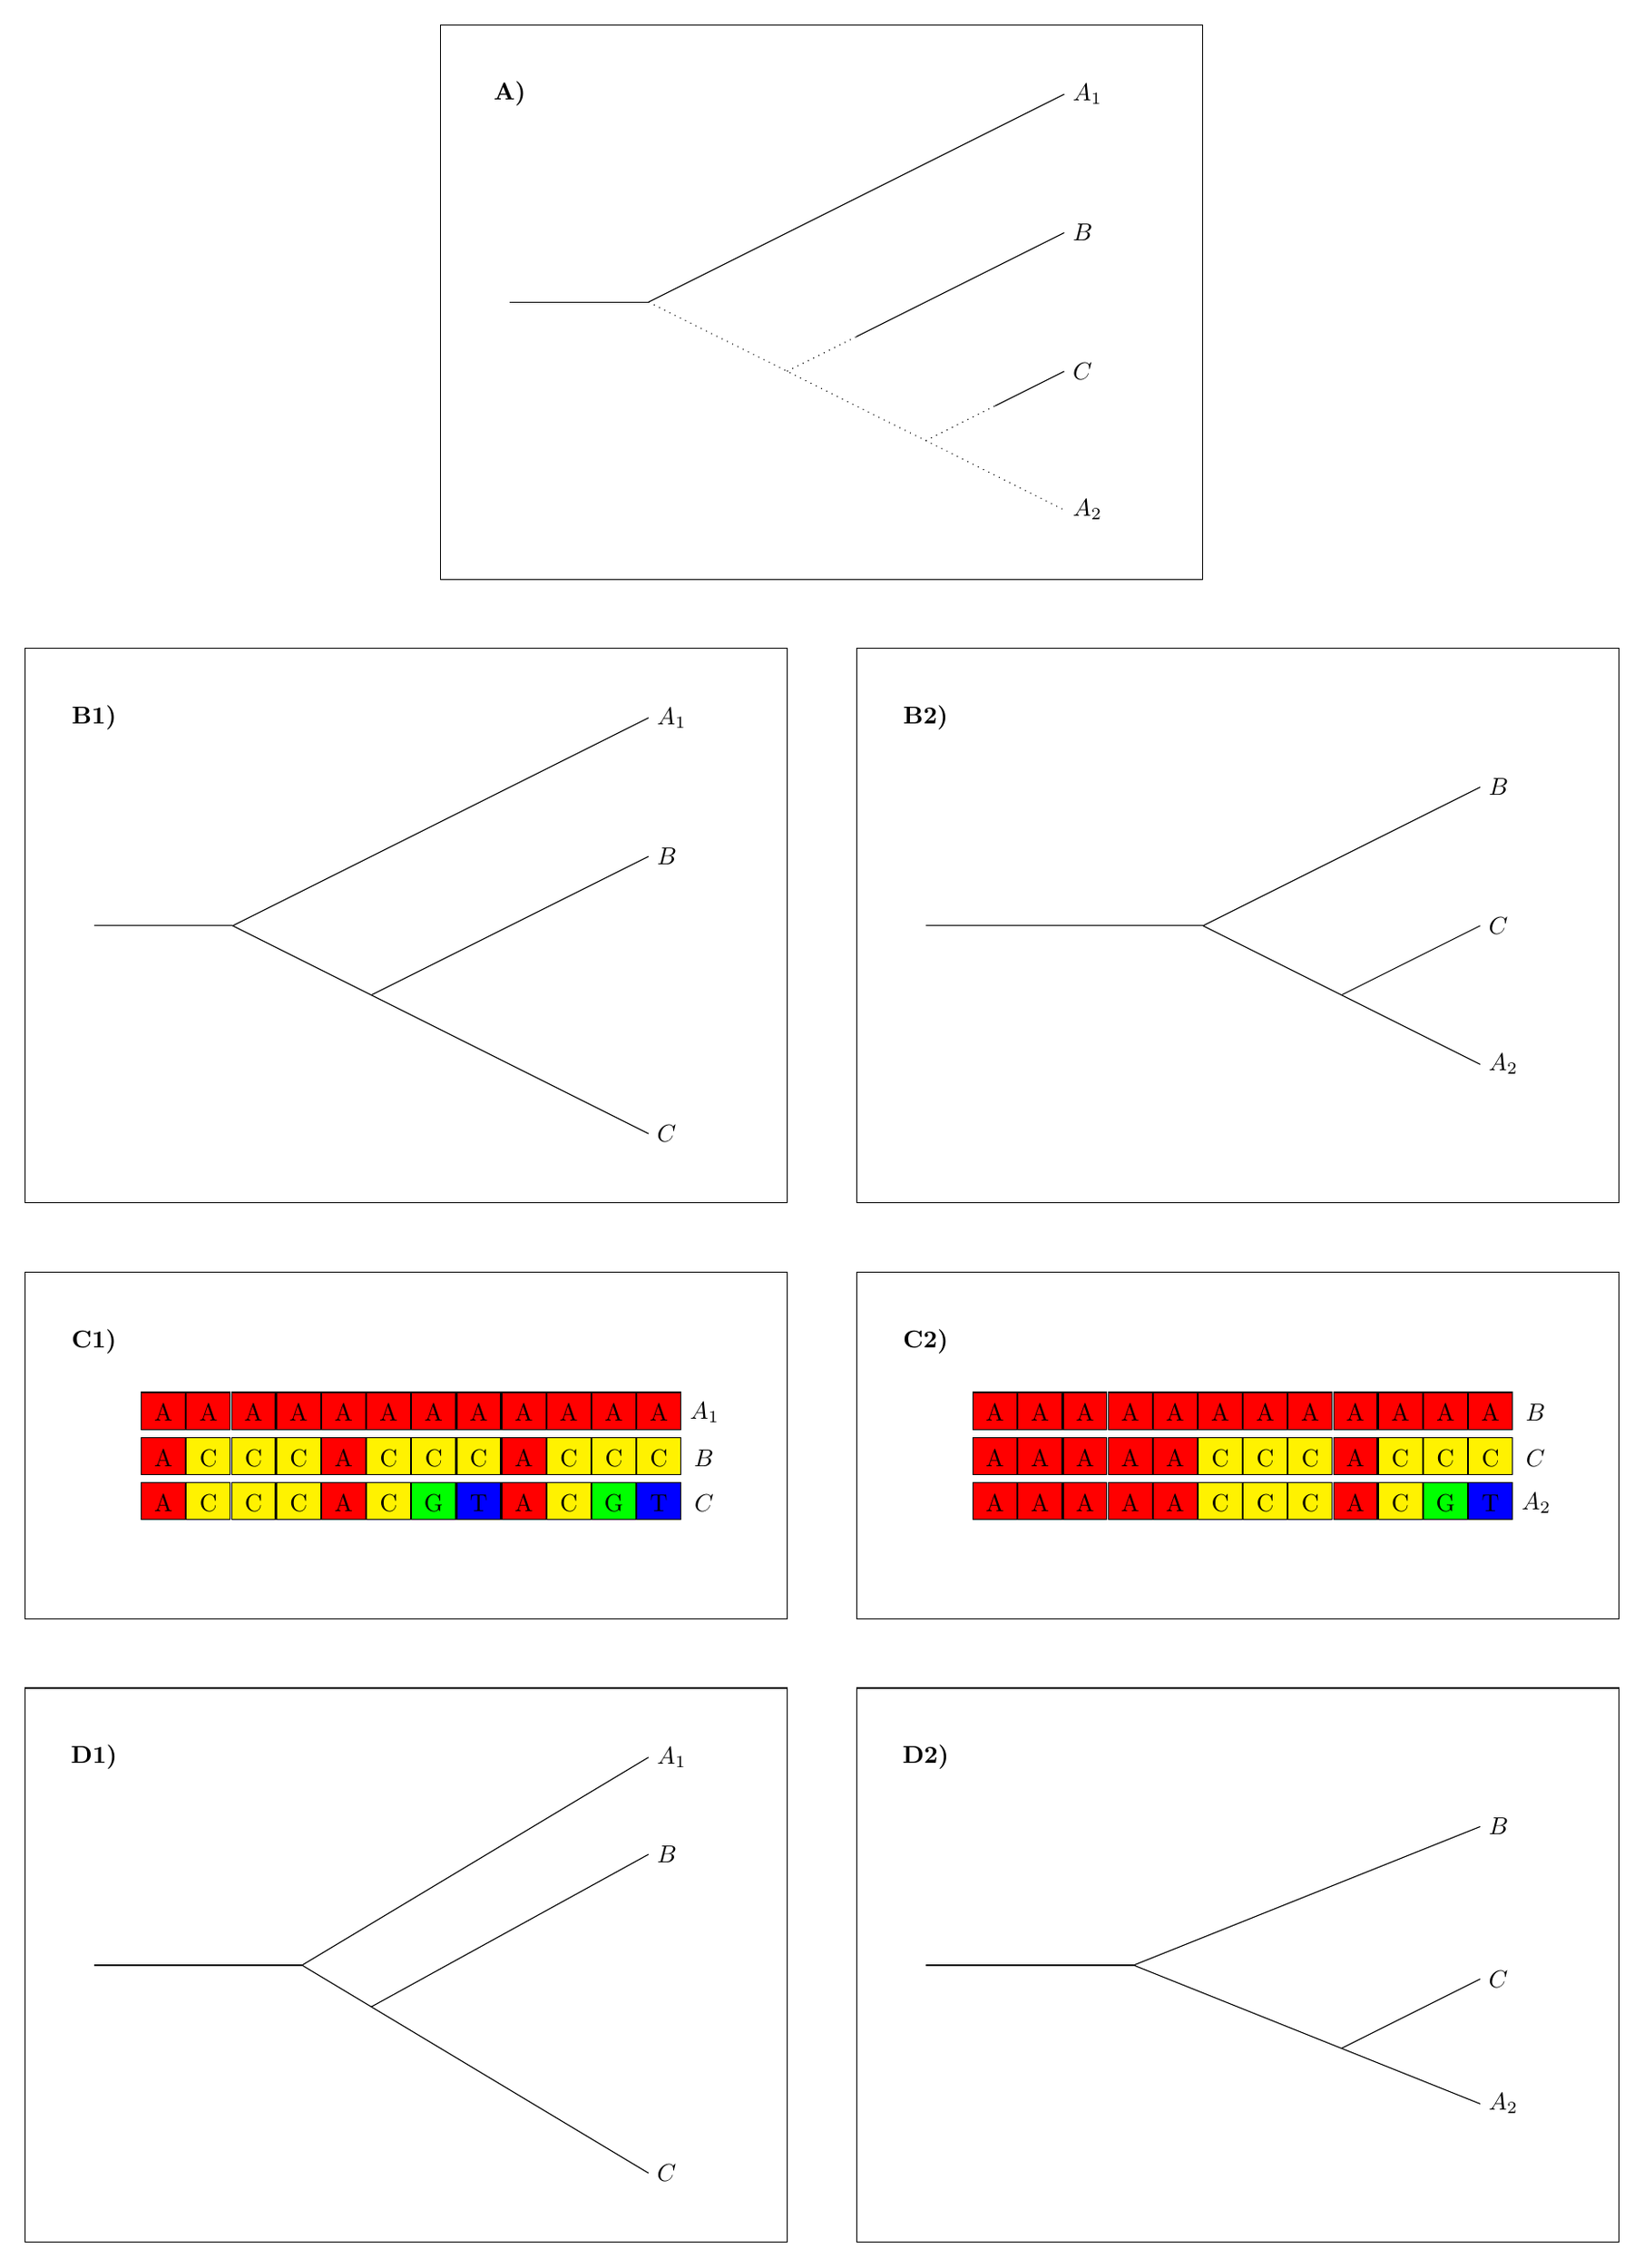
\begin{tikzpicture} 

    % Incipient species tree
    \begin{scope}[shift={(0,0)}] 

      \node[font = \bf] at (0, 0) {A)};
      \draw (-1,1) rectangle (10,-7);

      % Drawing of the phylogeny
      \begin{scope}[shift={(0,-3)}] 
        \draw (0, 0) -- (2,  0); % stem 
        \draw (2, 0) -- (8,  3) node[anchor=west] {$A_1$};
        \draw[dotted] (4,  -1) -- (5, -0.5); \draw (5, -0.5) -- (8, 1) node[anchor=west] {$B$};
        \draw[dotted] (6,  -2) -- (7, -1.5); \draw (7, -1.5) -- (8, -1) node[anchor=west] {$C$};
        \draw[dotted] (2,0) -- (8, -3) node[anchor=west] {$A_2$};
      \end{scope} % Drawing of the phylogeny

    \end{scope}


    % Species tree, oldest
    \begin{scope}[shift={(-6,-9)}] 

      \node[font = \bf] at (0.0, 0  ) {B1)};
      \draw (-1,1) rectangle (10,-7);

      % Drawing of the species tree, oldest
      \begin{scope}[shift={(0,-3)}] 
        \draw (0, 0) -- (2,  0); % stem 
        \draw (2, 0) -- (8,  3) node[anchor=west] {$A_1$};
        \draw (4,  -1) -- (8, 1) node[anchor=west] {$B$};
        \draw (2,0) -- (8, -3) node[anchor=west] {$C$};
      \end{scope} % Drawing of the species tree, oldest

    \end{scope}


    % Species tree, youngest
    \begin{scope}[shift={( 6,-9)}] 

      \node[font = \bf] at (0, 0) {B2)};
      \draw (-1,1) rectangle (10,-7);

      % Drawing of the species tree, youngest
      \begin{scope}[shift={(0,-3)}] 
        \draw (0, 0) -- (4,  0); % stem 
        \draw (4, 0) -- (8,  2) node[anchor=west] {$B$};
        \draw (6,-1) -- (8,  0) node[anchor=west] {$C$};
        \draw (4, 0) -- (8, -2) node[anchor=west] {$A_2$};
      \end{scope} % Drawing of the species tree, youngest

    \end{scope}

    % Alignment, oldest
    \begin{scope}[shift={(-6,-18)}] 

      \node[font = \bf] at (0.0, 0  ) {C1)};
      \draw (-1,1) rectangle (10,-4);

      % Drawing of the alignment
      \begin{scope}[shift={(1,-1)}, text width = 4mm, text height = 3mm, align = center, scale = 1.3] 

        \node[draw, fill = red   ] at (0.0, 0  ) {A};
        \node[draw, fill = red   ] at (0.5, 0  ) {A};
        \node[draw, fill = red   ] at (1.0, 0  ) {A};
        \node[draw, fill = red   ] at (1.5, 0  ) {A};
        \node[draw, fill = red   ] at (2.0, 0  ) {A};
        \node[draw, fill = red   ] at (2.5, 0  ) {A};
        \node[draw, fill = red   ] at (3.0, 0  ) {A};
        \node[draw, fill = red   ] at (3.5, 0  ) {A};
        \node[draw, fill = red   ] at (4.0, 0  ) {A};
        \node[draw, fill = red   ] at (4.5, 0  ) {A};
        \node[draw, fill = red   ] at (5.0, 0  ) {A};
        \node[draw, fill = red   ] at (5.5, 0  ) {A};
        \node[                   ] at (6.0, 0  ) {$A_1$};

        \node[draw, fill = red   ] at (0.0, -0.5) {A};
        \node[draw, fill = yellow] at (0.5, -0.5) {C};
        \node[draw, fill = yellow] at (1.0, -0.5) {C};
        \node[draw, fill = yellow] at (1.5, -0.5) {C};
        \node[draw, fill = red   ] at (2.0, -0.5) {A};
        \node[draw, fill = yellow] at (2.5, -0.5) {C};
        \node[draw, fill = yellow] at (3.0, -0.5) {C};
        \node[draw, fill = yellow] at (3.5, -0.5) {C};
        \node[draw, fill = red   ] at (4.0, -0.5) {A};
        \node[draw, fill = yellow] at (4.5, -0.5) {C};
        \node[draw, fill = yellow] at (5.0, -0.5) {C};
        \node[draw, fill = yellow] at (5.5, -0.5) {C};
        \node[                   ] at (6.0, -0.5) {$B$};

        \node[draw, fill = red] at (0.0, -1.0) {A};
        \node[draw, fill = yellow] at (0.5, -1.0) {C};
        \node[draw, fill = yellow] at (1.0, -1.0) {C};
        \node[draw, fill = yellow] at (1.5, -1.0) {C};
        \node[draw, fill = red   ] at (2.0, -1.0) {A};
        \node[draw, fill = yellow] at (2.5, -1.0) {C};
        \node[draw, fill = green ] at (3.0, -1.0) {G};
        \node[draw, fill = blue  ] at (3.5, -1.0) {T};
        \node[draw, fill = red   ] at (4.0, -1.0) {A};
        \node[draw, fill = yellow] at (4.5, -1.0) {C};
        \node[draw, fill = green ] at (5.0, -1.0) {G};
        \node[draw, fill = blue  ] at (5.5, -1.0) {T};
        \node[                   ] at (6.0, -1.0) {$C$};

      \end{scope} % Drawing of the alignment

    \end{scope}

    % Alignment, youngest
    \begin{scope}[shift={(6,-18)}] 

      \node[font = \bf] at (0.0, 0  ) {C2)};
      \draw (-1,1) rectangle (10,-4);

      % Drawing of the alignment
      \begin{scope}[shift={(1,-1)}, text width = 4mm, text height = 3mm, align = center, scale = 1.3] 

        \node[draw, fill = red   ] at (0.0, 0  ) {A};
        \node[draw, fill = red   ] at (0.5, 0  ) {A};
        \node[draw, fill = red   ] at (1.0, 0  ) {A};
        \node[draw, fill = red   ] at (1.5, 0  ) {A};
        \node[draw, fill = red   ] at (2.0, 0  ) {A};
        \node[draw, fill = red   ] at (2.5, 0  ) {A};
        \node[draw, fill = red   ] at (3.0, 0  ) {A};
        \node[draw, fill = red   ] at (3.5, 0  ) {A};
        \node[draw, fill = red   ] at (4.0, 0  ) {A};
        \node[draw, fill = red   ] at (4.5, 0  ) {A};
        \node[draw, fill = red   ] at (5.0, 0  ) {A};
        \node[draw, fill = red   ] at (5.5, 0  ) {A};
        \node[                   ] at (6.0, 0  ) {$B$};

        \node[draw, fill = red   ] at (0.0, -0.5) {A};
        \node[draw, fill = red   ] at (0.5, -0.5) {A};
        \node[draw, fill = red   ] at (1.0, -0.5) {A};
        \node[draw, fill = red   ] at (1.5, -0.5) {A};
        \node[draw, fill = red   ] at (2.0, -0.5) {A};
        \node[draw, fill = yellow] at (2.5, -0.5) {C};
        \node[draw, fill = yellow] at (3.0, -0.5) {C};
        \node[draw, fill = yellow] at (3.5, -0.5) {C};
        \node[draw, fill = red   ] at (4.0, -0.5) {A};
        \node[draw, fill = yellow] at (4.5, -0.5) {C};
        \node[draw, fill = yellow] at (5.0, -0.5) {C};
        \node[draw, fill = yellow] at (5.5, -0.5) {C};
        \node[                   ] at (6.0, -0.5) {$C$};

        \node[draw, fill = red   ] at (0.0, -1.0) {A};
        \node[draw, fill = red   ] at (0.5, -1.0) {A};
        \node[draw, fill = red   ] at (1.0, -1.0) {A};
        \node[draw, fill = red   ] at (1.5, -1.0) {A};
        \node[draw, fill = red   ] at (2.0, -1.0) {A};
        \node[draw, fill = yellow] at (2.5, -1.0) {C};
        \node[draw, fill = yellow] at (3.0, -1.0) {C};
        \node[draw, fill = yellow] at (3.5, -1.0) {C};
        \node[draw, fill = red   ] at (4.0, -1.0) {A};
        \node[draw, fill = yellow] at (4.5, -1.0) {C};
        \node[draw, fill = green ] at (5.0, -1.0) {G};
        \node[draw, fill = blue  ] at (5.5, -1.0) {T};
        \node[                   ] at (6.0, -1.0) {$A_2$};

      \end{scope} % Drawing of the alignment

    \end{scope}



    % Estimated species tree, oldest
    \begin{scope}[shift={(-6,-24)}] 

      \node[font = \bf] at (0, 0) {D1)};
      \draw (-1,1) rectangle (10,-7);

      \begin{scope}[shift={(0,-3)}] 
        \draw (0, 0) -- (3,  0);
        \draw (3, 0) -- (8, 3) node[anchor=west] {$A_1$};
        \draw (4,-0.6) -- (8, 1.6) node[anchor=west] {$B$};
        \draw (3, 0) -- (8,-3) node[anchor=west] {$C$};
      \end{scope}

    \end{scope}


    % Estimated species tree, youngest
    \begin{scope}[shift={(6,-24)}] 

      \node[font = \bf] at (0, 0) {D2)};
      \draw (-1,1) rectangle (10,-7);

      \begin{scope}[shift={(0,-3)}] 
        \draw (0, 0) -- (3,  0);
        \draw (3, 0) -- (8,  2) node[anchor=west] {$B$};
        \draw (6,-1.2) -- (8, -0.2) node[anchor=west] {$C$};
        \draw (3, 0) -- (8, -2) node[anchor=west] {$A_2$};
      \end{scope}

    \end{scope}

  \end{tikzpicture}
} % End of create_figure_experiment definition
%%%%%%%%%%%%%%%%%%%%%%%%%%%%%%%%%%%%%%%%%%%%%%%%%%%%%%%%%%%%%%%%%%%%%%%%%%%%%%%%




%%%%%%%%%%%%%%%%%%%%%%%%%%%%%%%%%%%%%%%%%%%%%%%%%%%%%%%%%%%%%%%%%%%%%%%%%%%%%%%%
% Create the TikZ picture of fig:sampling
%%%%%%%%%%%%%%%%%%%%%%%%%%%%%%%%%%%%%%%%%%%%%%%%%%%%%%%%%%%%%%%%%%%%%%%%%%%%%%%%
\newcommand{\CreateTikzFigureSampling} {

  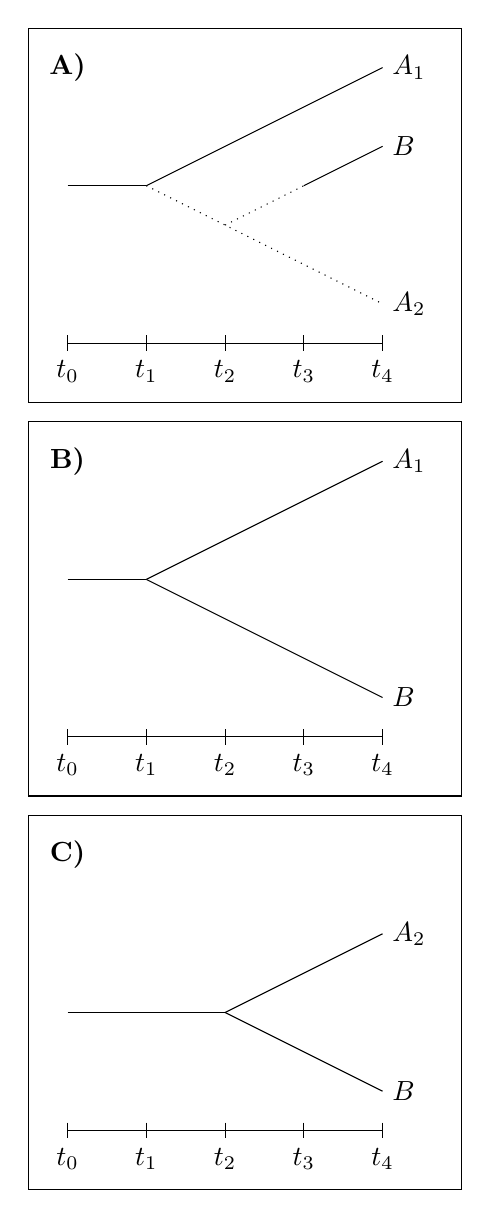
\begin{tikzpicture}[scale = 0.5] 

    \begin{scope}[shift={(0,0)}] 

      \node[font = \bf] at (0, 0) {A)};
      \draw (-1,1) rectangle (10,-8.5);

      % Drawing of the phylogeny
      \begin{scope}[shift={(0,-3)}] 
        \draw (0, 0) -- (2,  0);
        \draw (2, 0) -- (8,  3) node[anchor=west] {$A_1$};
        \draw[dotted] (2, 0) -- (8, -3) node[anchor=west] {$A_2$};
        \draw[dotted] (4, -1) -- (6, 0);
        \draw (6, 0) -- (8, 1) node[anchor=west] {$B$};
        % time scale
        \draw (0, -4) -- (8,  -4);
        \draw (0, -3.8) -- (0,  -4.2) node[anchor=north] {$t_0$};
        \draw (2, -3.8) -- (2,  -4.2) node[anchor=north] {$t_1$};
        \draw (4, -3.8) -- (4,  -4.2) node[anchor=north] {$t_2$};
        \draw (6, -3.8) -- (6,  -4.2) node[anchor=north] {$t_3$};
        \draw (8, -3.8) -- (8,  -4.2) node[anchor=north] {$t_4$};
      \end{scope} % Drawing of the phylogeny

    \end{scope}
    \begin{scope}[shift={(0, -10)}] 

      \node[font = \bf] at (0, 0) {B)};
      \draw (-1,1) rectangle (10,-8.5);

      % Drawing of the phylogeny
      \begin{scope}[shift={(0,-3)}] 
        \draw (0, 0) -- (2,  0);
        \draw (2, 0) -- (8,  3) node[anchor=west] {$A_1$};
        \draw (2, 0) -- (8, -3) node[anchor=west] {$B$};
        % time scale
        \draw (0, -4) -- (8,  -4);
        \draw (0, -3.8) -- (0,  -4.2) node[anchor=north] {$t_0$};
        \draw (2, -3.8) -- (2,  -4.2) node[anchor=north] {$t_1$};
        \draw (4, -3.8) -- (4,  -4.2) node[anchor=north] {$t_2$};
        \draw (6, -3.8) -- (6,  -4.2) node[anchor=north] {$t_3$};
        \draw (8, -3.8) -- (8,  -4.2) node[anchor=north] {$t_4$};
      \end{scope} % Drawing of the phylogeny

    \end{scope}
    \begin{scope}[shift={(0,-20)}] 

      \node[font = \bf] at (0, 0) {C)};
      \draw (-1,1) rectangle (10,-8.5);

      % Drawing of the phylogeny
      \begin{scope}[shift={(0,-3)}] 
        \draw (0, -1) -- (4, -1) ;
        \draw (4, -1) -- (8, -3) node[anchor=west] {$B$};
        \draw (4, -1) -- (8,  1) node[anchor=west] {$A_2$};
        % time scale
        \draw (0, -4) -- (8,  -4);
        \draw (0, -3.8) -- (0,  -4.2) node[anchor=north] {$t_0$};
        \draw (2, -3.8) -- (2,  -4.2) node[anchor=north] {$t_1$};
        \draw (4, -3.8) -- (4,  -4.2) node[anchor=north] {$t_2$};
        \draw (6, -3.8) -- (6,  -4.2) node[anchor=north] {$t_3$};
        \draw (8, -3.8) -- (8,  -4.2) node[anchor=north] {$t_4$};
      \end{scope} % Drawing of the phylogeny

    \end{scope}
  \end{tikzpicture}

} % End of create_figure_experiment definition
%%%%%%%%%%%%%%%%%%%%%%%%%%%%%%%%%%%%%%%%%%%%%%%%%%%%%%%%%%%%%%%%%%%%%%%%%%%%%%%%



% Use double spacing
\usepackage{setspace}
\doublespacing

\usepackage{listings}
\usepackage{hyperref}
\usepackage{todonotes}
\usepackage{verbatim}
\usepackage{pgf}
\usepackage{bm}

% TikZ and friends
\usepackage{tikz}
\usepackage{tkz-graph}
\usepackage{pgf}
\usetikzlibrary{arrows,automata}

% Style of listings
% From http://r.789695.n4.nabble.com/How-to-nicely-display-R-code-with-the-LaTeX-package-listings-tp4648110.html
\usepackage{fancyvrb} 
\definecolor{codegreen}{rgb}{0,0.6,0}
\definecolor{codegray}{rgb}{0.5,0.5,0.5}
\definecolor{codepurple}{rgb}{0.58,0,0.82}
\definecolor{backcolor}{rgb}{0.95,0.95,0.92}
\lstdefinestyle{mystyle}{
  language=R,% set programming language
  basicstyle=\ttfamily\small,% basic font style
  commentstyle=\color{gray},% comment style
  % numbers=left,% display line numbers on the left side
  numberstyle=\scriptsize,% use small line numbers
  numbersep=10pt,% space between line numbers and code
  tabsize=2,% sizes of tabs
  showstringspaces=false,% do not replace spaces in strings by a certain character
  captionpos=b,% positioning of the caption below
  breaklines=true,% automatic line breaking
  escapeinside={(*}{*)},% escaping to LaTeX
  fancyvrb=true,% verbatim code is typset by listings
  extendedchars=false,% prohibit extended chars (chars of codes 128--255)
  alsoletter={.<-},% becomes a letter
  alsoother={$},% becomes other
  otherkeywords={!=, ~, $, \&, \%/\%, \%*\%, \%\%, <-, <<-, /},% other keywords
  deletekeywords={c}% remove keywords 
}
\lstset{style=mystyle}

% Adds numbered lines
\usepackage{lineno}
\linenumbers

\begin{document}

\maketitle

\begin{abstract}

  % From 'How to construct a Nature summary paragraph'

  % A short abstract of fewer than 200 words is acceptable.

  % One or two sentences providing a basic
  % introduction to the field,
  % comprehensible to a scientist in any discipline.
  The tools for reconstructing phylogenetic relationships between taxonomic 
  units (e.g. species) have become very advanced in the last two decades. 

  % Two to three sentences of
  % more detailed background, comprehensible to
  % scientists in related disciplines.
  Among the most popular tools are Bayesian approaches, such as BEAST, MrBayes and RevBayes, 
  that use efficient tree sampling routines to create a posterior probability distribution 
  of the phylogenetic tree. 
  A feature of these approaches is the possibility to incorporate 
  known or hypothesized structure of the phylogenetic tree through the tree prior. 
  It has been shown that the effect of the prior on the posterior distribution 
  of trees can be substantial. 

  % One sentence clearly stating the general
  % problem being addressed by this particular
  % study.
  Currently implemented tree priors assume that speciation is instantaneous,
  where we know that speciation can be a gradual process.

  % One sentence summarising the main
  % result (with the words “here we show”
  % their equivalent).
  Here we explore the effects of ignoring 
  the protractedness of the speciation process with an extensive simulation study. 

  % Two or three sentences explaining what
  % the main result reveals in direct
  % comparison to what was thought to be the case
  % previously, or how the main result adds to
  % previous knowledge.

  % One or two sentences to put the results into a
  % more general context.


  % Two or three sentences to provide a
  % broader perspective, readily comprehensible
  % to a scientist in any discipline, may be included
  % in the first paragraph if the editor considers that the accessibility of the paper is significantly enhanced
  % by their inclusion. Under these circumstances, the length of the paragraph can be up to 300 words.
  % (The above example is 190 words without the final section, and 250 words with it).
  We conclude that ...

  % Does not seem to fit here: 
  %  
  % We simulate protracted phylogenies using the protracted birth-death process 
  % and then simulate sequence alignments according to a substitution model and clock model. 
  % We then use BEAST to infer the phylogeny from these alignments using the standard 
  % birth-death prior that assumes instantaneous speciation. We compare the 
  % inferred tree to the simulated tree, and find that ....
  % 
  % Furthermore, we identify an important issue related to protracted speciation. 
  % Because the tree produced by the protracted birth-death process 
  % is not necessarily monophyletic, we cannot speak of "the" species tree. 
  % Instead we have to sample among the incipient species to represent species. 
  % We show that different ways of sampling the representative species results in ....


\end{abstract}

{\bf Keywords:} computational biology, evolution, phylogenetics, prior choice

%%%%%%%%%%%%%%%%%%%%%%%%%%%%%%%%%%%%%%%%%%%%%%%%%%%%%%%%%%%%%%%%%%%%%%%%%%%%%%%%%%%%%%
\section{Introduction}
%%%%%%%%%%%%%%%%%%%%%%%%%%%%%%%%%%%%%%%%%%%%%%%%%%%%%%%%%%%%%%%%%%%%%%%%%%%%%%%%%%%%%%

The computational tools a contemporary phylogeneticist has at his/her disposal
goes beyond the wildest imagination of those living two decades ago. 
Advances in computational power allowed the first cladograms to be inferred 
from DNA alignments in [some year, some ref]. The first time-trees were
published in [some year, some ref]. Thanks to the addition of effective sampling
methods, the first Bayesian tools appeared in [some year, some ref], allowing
for unprecedented flexibility in the setup of a phylogenetic model.

Currently, the most popular Bayesian phylogenetics tools are BEAST [ref],  
MrBayes [ref] and RevBayes [ref]. Each of these use efficient tree sampling 
routines to create a posterior probability distribution of the to-be-inferred 
phylogenetic tree. But next to the computational speed, they also allow
to incorporate known or hypothesized structure of the phylogenetic 
tree-to-be-inferred through the model priors.

The model prior most relevant here, is the tree prior. The tree prior
embodies the assumed speciation model. Each speciation model has a
different expected branch length distribution. It has been shown 
[Moeller, du Plessis, Stadler. 2018] that the effect of the prior on the posterior distribution 
of trees can be substantial. 

All of the currently implemented tree priors assume that speciation is 
instantaneous, where we know that speciation can be a gradual process.
The protracted birth-death (PBD) model, an extension of 
the (constant-rate) birth-death (BD) model, incorporates this idea.
In the PBD model, a branching event does not give rise to a new species, but to
a new species-to-be, called an incipient species. Such an incipient
species may go extinct, or finish its speciation to become a good species.

Although we know speciation takes time, all of our theoretical 
phylogenetic modeling tools ignore this fact. One reason may be to ease
computation, enabling researchers to work on bigger phylogenies (with
more power statistical power) instead. Additionally, speciation being
protracted is only playing a role in the present. As seen from the present,
all older species have finished speciation, as we -by definition- recognize
these species as such. 

There are problems with ignoring protracted speciation. A very pragmatic
example is the conservation of an underestimated amount of species. 
But from a more theoretical perspective, the
observed decline of speciation rate in time (excluding the contemporary human-driven
mass extinction event) may be explained by these new species not being 
recognized yet. Another problem is that the most recent common 
ancestor (MRCA) of a young species duo is estimated 
too close to the present, as in the BD model a species can be 
ultra-young (as speciation is assumed to be instantaneous), 
where the PBD model will place these MRCAs
further back in time (as two events need to have finished completion).

From a theoretical point of view, there is another reason why protracted
speciation has not yet become a member of our toolbox: there is no framework
where it fits in: a framework assumes either an analysis at the species or
subspecies level. When picking a tool that does its analysis at the
species level, there is no protocol how to select which incipient species
gets to represent the full species it is still a member of. When picking
a tool at the sub-species level, the incipient state disappears as a
sub-species lineage, and the process degrades to an ordinary birth-death 
process.

This exploratory research's goal is to produce a 
useful and balanced data set, that quantifies the inference error 
we make from choosing the incorrect prior. In this context, 
we measure the error made on PBD phylogenies, when using a BD prior.

The parameter space the data set explores is inspired on 
[Etienne et al, 2014] for two reasons: (1) the academic
reason of being able to compare results, and (2) the practical
reason that the simulated phylogies will have enough taxa to
be informative, but not too big to be computationally overdemanding.
This research uses a complete superset of those parameter settings.
For the speciation initiation rate, we'll use $0.1$, $0.5$ and $1.0$ 
speciation initiation events per (good species) lineage per time unit, 
extending the set of
values used from one ($0.5$) to three. 
The speciation completion
rates used are $0.1$, $0.3$, $1.0$ and $10^6$ speciation completion
events per (incipient species) lineage per time unit, in which only
the last value is added as a computational proxy for infinity, which
makes the experiment fall back to a Birth-Death model (as speciation
is again instantaneous), allowing to measure the baseline error.
The extinction rates used are $0.0$, $0.1$, $0.2$ and $0.4$ 
extinction events per (good or incipient) lineage per time unit,
in which $0.4$ is a new extinction rate.
We investigate these parameters in a factorial fashion, except for
(1) those combinations in which the extinction rate equals or exceeds
the speciation initiation rate, and (2) the difference between
speciation initiation rate and extinction rate exceeds 0.8. This is
done to prevent overly taxon-poor and taxon-rich phylogenies respectively.

From each biological parameter set, a protracted birth-death tree is simulated,
with the same crown age as [Etienne et al., 2014] of 15 million years. 
Each protracted birth-death tree uses a different random number
generatior seed, and thus will be unique, resulting in a balanced 
data set. 

From an incipient species tree, we sample a species tree
by picking either the youngest or oldest
species-to-be to represent the full species.
We use either sampling method in 50\% of all cases. We chose not to use
a random species-to-be to represent a full species as to maximize variance
in this aspect. Note that only in few cases (when speciation completion rate
is low) the sampling method has an effect on the branch length distribution
of the sampled species tree, as this requires a very specific scenario.

From a species tree, we simulate a DNA alignment that has the same history
as the phylogeny. The nucleotides of the DNA alignment follow a JC69
nucleotide substitution model, in which all nucleotide-to-nucleotide transitions
are equally likely. Although this may seem as a simplification, in our Bayesian
inference (see below) we can use this exact site model as a prior, which we 
know is the truth.
The DNA sequence length and mutation rate was chosen as such to provide one
nucleotide change per 1000 years per lineage. As our time unit is in 
millions of years, and our crown age is 15 million years,
this equates to a rate of $\frac{1000}{15}$ nucleotide substitutions 
changes per time unit per lineage. To provide for each substitution being unique,
we simulate as much DNA nucleotides as expected mutations, which equals the
nucleotide substitution rate times the crown age, which equals 15K. As this
mutation rate is constant over all branches, it in effect follows a strict 
clock model, which we will specify as the known clock model prior later.

From an alignment, we run a Bayesian analysis and create a posterior, 
using the phylogetic tool BEAST2. We assume a
JC69 nucleotide substitution (as we do use that), a strict clock model with 
the same fixed rate as used in the simulation of the alignment (as
we have that) and a Birth-Death tree prior (as this simplification is the goal
of this research). Additionally, we assume a MRCA prior with a normal distribution
with a mean of the crown age, and a standard deviation of 0.001 time units. 0.001
time units equates to 1000 years, which is the same resolution as which the
alignment is created. After discarding a burn-in of 10\%, the MCMC algorithm must 
result in an ESS of the posterior of at least 200 and the MCMC sampling interval is 
chosen as such that this is the case for all simulations. For simulations
with an ESS below 200, their MCMC sampling interval is doubled up until
the ESS exceeds 200. 

We realize there will be an unavoidable bias in our data set: the MCMC
algorithm will produce phylogenies that are representative for the joint
likelihood of (correct) site model, (correct) clock model and 
(incorrect) (Birth-Death) speciation model. This will
warp the distribution of phylogenies somewhat towards the incorrect
speciation model: branch length distributions that are likely in the
Birth-Death model will be relatively overrepresented. We expect
this bias to be systematic, equally affecting distributions
of identical speciation completion rates, and symptomatic
of using contemporary tools.

Each posterior's phylogeny is compared to the (sampled) species tree.
To quantify the difference between two phylogenies, the nLTT statistic
is used. The nLTT statistic equates to the area between the normalized
lineages-through-time-plots of two phylogenies, which will be a value between 
zero (for identical phylogenies) and one. As the nLTT statistic increases
when phylogenies get increasingly different, we use the nLTT statistic
as a measure of inference error. Comparing the one (sampled) species tree
with each of the posterior's species trees, a distribution nLTT statistics
is created. 

We predict that nLTT statistic values increase 
with an increasing protractednedness (that is, a low speciation completion rate),
but we cannot predict the the extent of this error, as it has never been 
measured [NOTE: this may be easy to change: Etienne \& Rosindel 2012 show the equations
for the expected number of lineages through time. I think I may be able to pull
of a prediction here, by fitting a BD curve on a PBD curve with a minimized error,
but research would be needed to investigate that].

The data set produced by this exploratory research will consist out of two files:
one containing raw data, the other summarized data. 
A data file should be convenient to handle, thus as an upper limit for this data set's size, 
we use the maximum size of a table (called a data frame) of the R programming 
language. Within R, such a table may have maximally $2^{32}-1$ cells and occupy
less then 2 gigabytes in memory. 
The raw data file will contain parameters and 1000 nLTT statistics values.
Each row will contain the parameter set and these nLTT statistics.
From the constraints of the R programming language, this allows for 40K rows. 
The file with the summarized data will provide summary statistics of the raw
data. Each row will contain a parameter set, summary statistics and other
measurements. See the appendix, chapter 'Data set specifications', for the full list.

To visualize the data set, we will produce two figures.
The first figure will display the distribution 
of median nLTT statistics per combination of speciation initiation, speciation
completion and extinction rate. We will use the median nLTT statistic over 
summing nLTT statistic distributions, as we think this will give the cleanest
visualization [NOTE: I am unconvinced, wouldn't a violin plot would
be better?]. We will use the median nLTT statistic, instead of the mean, as
we expect the distribution of nLTT statistics not to be symmetrical. The distribution
of median nLTT statistics is displayed per biological parameter set in a box-plot,
to shown of that distribution as needed, without showing an overly amount of detail
regarding that distribution. 
The second figure will show the distribution of median nLTT statistics per expected
mean duration of speciation. The expected mean duration of parameter can be calculated
with equation 19 of [Etienne \& Rosidell 2012] and is a combination of the three
biological parameters combined to their relevant biological effect. Through these
points, we'll fit a straight line (we have no reason to expect an effect of
higher order) and a locally weighted scatterplot smoothing (LOESS) 
curve, which is a non-parametric fit to expose potential higher order effects.
Additionally, we'll draw a horizontal line to the average nLTT 
value (over all replicates) of those simulations with instantaneous speciation, 
which serves as a baseline of
the inference error made.

%%%%%%%%%%%%%%%%%%%%%%%%%%%%%%%%%%%%%%%%%%%%%%%%%%%%%%%%%%%%%%%%%%%%%%%%%%%%%%%%%%%%%%
\section{Results}
%%%%%%%%%%%%%%%%%%%%%%%%%%%%%%%%%%%%%%%%%%%%%%%%%%%%%%%%%%%%%%%%%%%%%%%%%%%%%%%%%%%%%%

\begin{figure}[!htbp]
  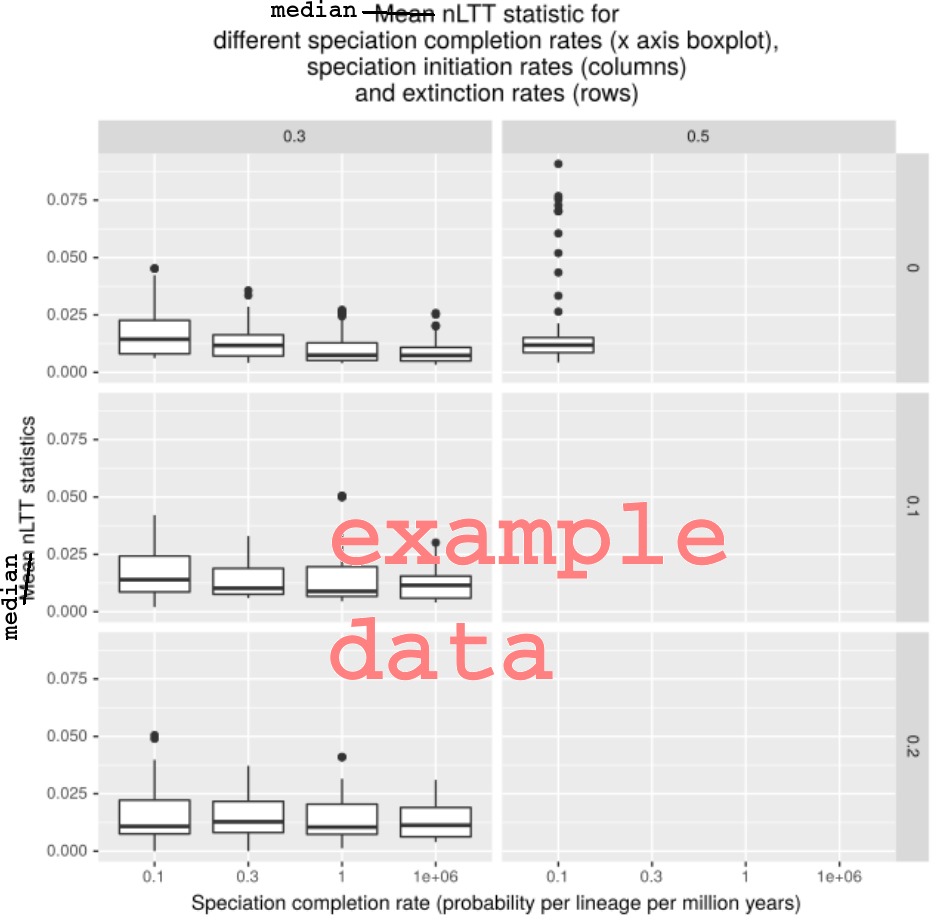
\includegraphics[width=0.8\textwidth]{nltt_stats_per_setup.png}
  \caption{
    median nLTT statistic distribution per parameter setting
  }
\end{figure}

\begin{figure}[!htbp]
  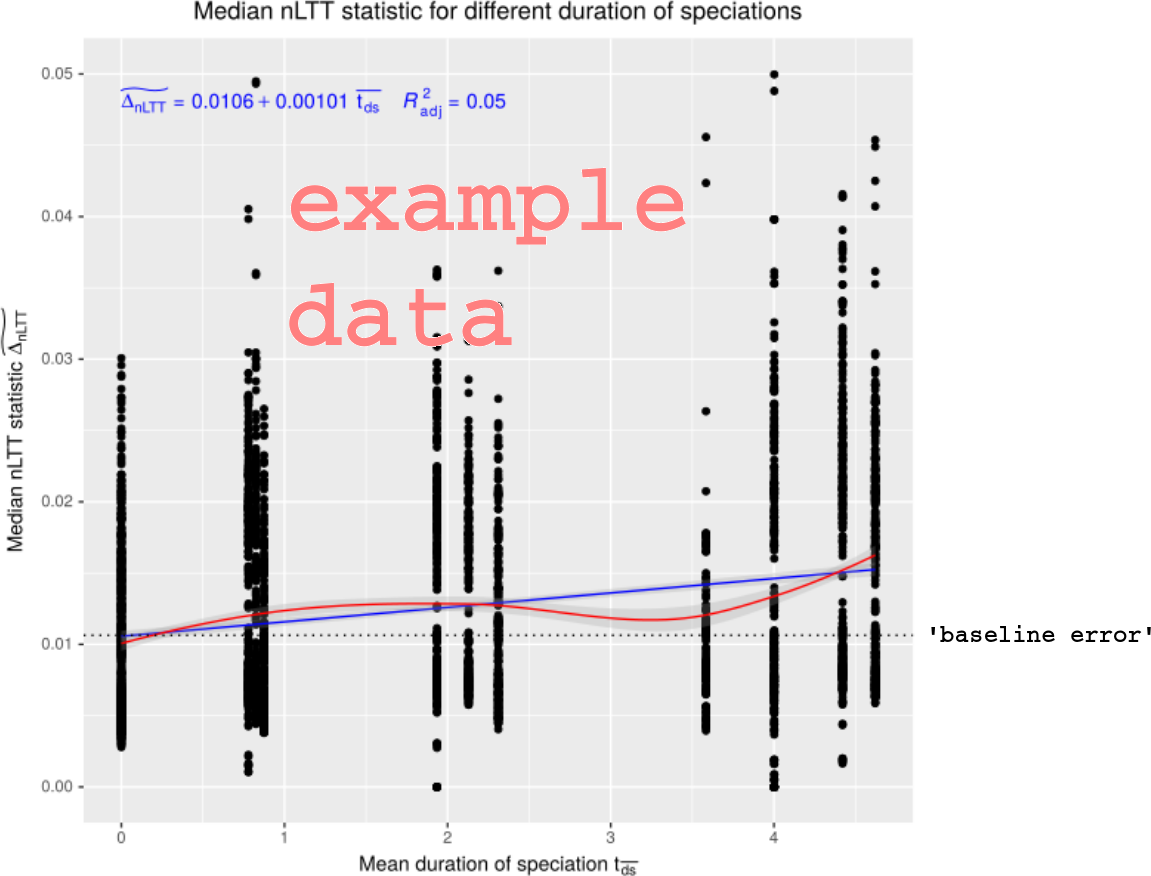
\includegraphics[width=0.8\textwidth]{nllt_stats_per_mean_dur_spec.png}
  \caption{
    median nLTT statistic distribution per mean duration of speciation
  }
\end{figure}

%%%%%%%%%%%%%%%%%%%%%%%%%%%%%%%%%%%%%%%%%%%%%%%%%%%%%%%%%%%%%%%%%%%%%%%%%%%%%%%%%%%%%%
\section{Glossary}
%%%%%%%%%%%%%%%%%%%%%%%%%%%%%%%%%%%%%%%%%%%%%%%%%%%%%%%%%%%%%%%%%%%%%%%%%%%%%%%%%%%%%%

% Please supply, as a separate list, the definitions of field-specific terms used in your article.

%%%%%%%%%%%%%%%%%%%%%%%%%%%%%%%%%%%%%%%%%%%%%%%%%%%%%%%%%%%%%%%%%%%%%%%%%%%%%%%%%%%%%%
\section{Acknowledgements}
%%%%%%%%%%%%%%%%%%%%%%%%%%%%%%%%%%%%%%%%%%%%%%%%%%%%%%%%%%%%%%%%%%%%%%%%%%%%%%%%%%%%%%

We would like to thank the Center for Information Technology of the University of Groningen for their support
and for providing access to the Peregrine high performance computing cluster.

%%%%%%%%%%%%%%%%%%%%%%%%%%%%%%%%%%%%%%%%%%%%%%%%%%%%%%%%%%%%%%%%%%%%%%%%%%%%%%%%%%%%%%
\section{Authors' contributions}
%%%%%%%%%%%%%%%%%%%%%%%%%%%%%%%%%%%%%%%%%%%%%%%%%%%%%%%%%%%%%%%%%%%%%%%%%%%%%%%%%%%%%%

%%%%%%%%%%%%%%%%%%%%%%%%%%%%%%%%%%%%%%%%%%%%%%%%%%%%%%%%%%%%%%%%%%%%%%%%%%%%%%%%%%%%%%
% Bibliography
%%%%%%%%%%%%%%%%%%%%%%%%%%%%%%%%%%%%%%%%%%%%%%%%%%%%%%%%%%%%%%%%%%%%%%%%%%%%%%%%%%%%%%
% MEE style
\bibliographystyle{mee}
\bibliography{article}
%%%%%%%%%%%%%%%%%%%%%%%%%%%%%%%%%%%%%%%%%%%%%%%%%%%%%%%%%%%%%%%%%%%%%%%%%%%%%%%%%%%%%%

%%%%%%%%%%%%%%%%%%%%%%%%%%%%%%%%%%%%%%%%%%%%%%%%%%%%%%%%%%%%%%%%%%%%%%%%%%%%%%%%%%%%%%
\appendix
%%%%%%%%%%%%%%%%%%%%%%%%%%%%%%%%%%%%%%%%%%%%%%%%%%%%%%%%%%%%%%%%%%%%%%%%%%%%%%%%%%%%%%

%%%%%%%%%%%%%%%%%%%%%%%%%%%%%%%%%%%%%%%%%%%%%%%%%%%%%%%%%%%%%%%%%%%%%%%%%%%%%%%%
\begin{table}
  \centering 
  \begin{tabular}{l l l}
    \hline
    Parameter             & Description & Values \\
    \hline
    \hline
    $b = b_g = b_i$       & Speciation initiation rate & 0.1, 0.5, 1.0 \\
    $\lambda$             & Speciation completion rate & 0.1, 0.3, 1.0, $10^6$ \\
    $\mu = \mu_g = \mu_i$ & Extinction rate & 0.0, 0.1, 0.2, 0.4 \\
    $t_c$                 & Crown age & 15 \\
    $\sigma_c$            & Standard deviation around crown age & 0.001 \\
    $M$                   & Sampling method & Youngest for odd $R_i$, oldest for even $R_i$ \\
    $r$                   & Mutation rate & $\frac{1000}{15}$ \\
    $l_a$                 & DNA alignment length & $15K$ \\
    $f_i$                 & MCMC sampling interval & 1K or more \\
    $R_i$                 & RNG seed incipient tree & 1 to 40K \\
    $R_a$                 & RNG seed alignment simulation & 1 to 40K \\
    $R_b$                 & RNG seed BEAST2 & 1 to 40K \\
    \hline
  \end{tabular}
  \caption{
    Overview of the 12 simulation parameters.
  }
  \label{table:simulation_parameters}
\end{table}
%%%%%%%%%%%%%%%%%%%%%%%%%%%%%%%%%%%%%%%%%%%%%%%%%%%%%%%%%%%%%%%%%%%%%%%%%%%%%%%%

%%%%%%%%%%%%%%%%%%%%%%%%%%%%%%%%%%%%%%%%%%%%%%%%%%%%%%%%%%%%%%%%%%%%%%%%%%%%%%%%
\begin{table}
  \centering 
  \begin{tabular}{l l}
    \hline
    $n$ & Description \\
    \hline
    \hline
    $12$   & simulation parameters \\
    $1000$ & nLTT statistic \\
    \hline
    $12$ & simulation parameters \\
    $1$ & expected duration of speciation (from Etienne \& Rosindell 2012) \\
    $1$ & number of taxa in incipient species tree (also: number of subspecies) \\
    $1$ & number of taxa in species tree (also: number of species) \\
    $1$ & mean nLTT statistic \\
    $1$ & median nLTT statistic \\
    $1$ & lower bound of 95\% HPD value of nLTT statistic \\
    $1$ & upper bound of 95\% HPD value of nLTT statistic \\
    $11$ & ESSes of all parameters estimated by BEAST2 (see specs below) \\
    \hline
  \end{tabular}
  \caption{
    Specification of the data sets. $n$ denotes the number
    of columns a certain item will occupy. Above the horizontal line,
    the content of the raw data file is specified, resulting in a table of 
    1012 columns and 40K rows. Below the horizontal line,
    the content of the summary data file specified, resulting in a table of
    40 columns and 40K rows.
  }
  \label{table:raw_data_set_specs}
\end{table}
%%%%%%%%%%%%%%%%%%%%%%%%%%%%%%%%%%%%%%%%%%%%%%%%%%%%%%%%%%%%%%%%%%%%%%%%%%%%%%%%

%%%%%%%%%%%%%%%%%%%%%%%%%%%%%%%%%%%%%%%%%%%%%%%%%%%%%%%%%%%%%%%%%%%%%%%%%%%%%%%%
\begin{table}
  \centering 
  \begin{tabular}{l l}
    \hline
    \# & Description \\
    \hline
    \hline
    1 & posterior \\
    2 & likelihood \\
    3 & prior \\
    4 & treeLikelihood \\
    5 & TreeHeight \\
    6 & BirthDeath \\
    7 & BDBirthRate \\
    8 & BDDeathRate \\
    9 & logP.mrca \\
    10 & mrcatime \\
    11 & clockRate \\
    \hline
  \end{tabular}
  \caption{
    Overview of the 11 BEAST2 estimated parameters
  }
  \label{table:estimated_parameters}
\end{table}
%%%%%%%%%%%%%%%%%%%%%%%%%%%%%%%%%%%%%%%%%%%%%%%%%%%%%%%%%%%%%%%%%%%%%%%%%%%%%%%%

\end{document}
